\documentclass{article}

\usepackage{fontspec}
\setmainfont{Open Sans-Regular}
\usepackage{tikz}
\usetikzlibrary{shapes.gates.logic.US}
\input{dft-tikz}
\definecolor{normalfillcolor}{gray}{0.7}
\setlength\paperwidth{30cm}
\setlength\hoffset{-2in}
\newdimen\zigzagvert
\zigzagvert=4mm % Connections first go this far down, then zig-zag to
                % their target.
\pagestyle{empty}

\begin{document}
\begin{tikzpicture}[
	rectangle/.style={fill=normalfillcolor, inner sep=5pt},
	node distance=2cm,
	every node/.style={outer sep=0pt,font=\Large},
]
% Input 1 ignored (would be input count).
\def\basicevent#1[#2](#3)#4{
        \node[rectangle, draw, #2, minimum height=5.5mm](#3box){#4};
        \node[circle, minimum width=12mm, fill=normalfillcolor, draw,
		anchor=north] at (#3box.south) (#3) {};
}
% Input 1: Text in triangle.
\def\transferevent#1[#2](#3)#4{
        \node[rectangle, draw, #2, minimum height=5.5mm](#3box){#4};
	\path[draw, fill=normalfillcolor] (#3box.south)
		-- ++(-8mm, -15mm) -- ++(16mm, 0) -- (#3box.south);
	\path (#3box.south) ++ (0, -15mm) node[anchor=south] (#3) {#1};
}
\def\orevent#1[#2](#3)#4{
        \node[rectangle, draw, #2, minimum height=5.5mm](#3box){#4};
        \node[or gate US, minimum width=12mm, logic gate inputs=#1, rotate=90, fill=normalfillcolor, draw, anchor=output] at (#3box.south) (#3) {};
}
\def\andevent#1[#2](#3)#4{
        \node[rectangle, draw, #2, minimum height=5.5mm](#3box){#4};
        \node[and gate US, minimum width=12mm, logic gate inputs=#1, rotate=90, fill=normalfillcolor, draw, anchor=output] at (#3box.south) (#3) {};
}
% Input 1: Blank for normal, M for mirrored.
\def\sparegate#1[#2](#3)#4{
        \node[spare#1, fill=normalfillcolor, draw, anchor=north, #2]
		(#3) {};
	\node[anchor=north] at (#3.north) (#3box) {#4};
}
% Input 1 ignored (for consistency).
\def\fdepgate#1[#2](#3)#4{
        \node[fdep, fill=normalfillcolor, draw, anchor=north, #2]
		(#3) {};
	\node[anchor=north] at (#3.north) (#3box) {#4};
}
% \connectZZ{G.input}{vert. distance}{child}.
% Draw a line from G.input down by 'vert. distance', then zig-zag to
% child.
\def\connectcust#1#2#3{
	\draw[-] (#1) -- ++(0,#2) -| (#3box);
}
% \connect{G.input}{child} (Note: Only for vertical connections).
\def\connect#1#2{
	\connectcust{#1}{-\zigzagvert}{#2};
}
	\orevent{nn}[](top){System}
	\andevent{nn}[below of=top, xshift=-58mm](CCSF){\begin{tabular}{c}
		Common cause\\seal failure\end{tabular}}
	\andevent{nn}[below of=top, xshift=58mm](SFI){\begin{tabular}{c}
		Seals fail\\independently\end{tabular}}
	\connect{top.input 1}{CCSF}
	\connect{top.input 2}{SFI}

	\basicevent [below of=CCSF, xshift=-23mm](CTF){\begin{tabular}{c}
		Contamination\\tape fails\end{tabular}}
	\basicevent [below of=CCSF, xshift=23mm](CCSF2){\begin{tabular}{c}
		Common cause\\seal failure\end{tabular}}
	\connect{CCSF.input 1}{CTF}
	\connect{CCSF.input 2}{CCSF2}

	\basicevent [below of=SFI, xshift=-45mm](MMSF){\begin{tabular}{c}
		Metal-to-metal\\seal fails\end{tabular}}
	\orevent{nn}[below of=SFI](CSF){\begin{tabular}{c}
		Compression\\seal failure\end{tabular}}
	\basicevent [below of=SFI, xshift=4cm](FPF){\begin{tabular}{c}
		Fused plug\\fails\end{tabular}}
	\connect{SFI.input 1}{MMSF}
	\connect{SFI.west}{CSF}
	\connect{SFI.input 2}{FPF}

	\basicevent [below of=CSF, xshift=-23mm](CS1){\begin{tabular}{c}
		Compression\\seal 1 fails\end{tabular}}
	\basicevent [below of=CSF, xshift=23mm](CS2){\begin{tabular}{c}
		Compression\\seal 1 fails\end{tabular}}
	\connect{CSF.input 1}{CS1}
	\connect{CSF.input 2}{CS2}
\end{tikzpicture}
\end{document}
